\documentclass[letterpaper,10pt]{article}
\usepackage{amsmath}
\usepackage{amsfonts}
\usepackage{amssymb}
\usepackage{graphicx}
\usepackage{siunitx}
\usepackage[left=1in,right=1in,top=1in,bottom=1in]{geometry}

\title{Notes on the Simulation of Broadband Sources}
\author{C.D. Clark III}

\begin{document}

\section{Background}
Broadband sources are light sources that contain a spectrum of wavelengths, and the total power of the source is distributed among the wavelengths. The distribution of power is called the ``power spectrum'',
and is most conveniently specified as function of wavelength. Let $p(\lambda)$ be the power spectrum for some broadband spectrum. The total power $P$ in the emitter is
\begin{equation}
  \label{eq:power_int}
  P = \int\limits_{0}^{\infty} p(\lambda) d\lambda
\end{equation}
The dimensions of $p$ must be power over length. If the wavelength is measured in \si{\nano\meter} and power is measured in \si{\watt}, the units
on $p$ will be \si{\watt\per\nano\meter}. These units are important for correctly simulating a broadband exposure.

\section{Modeling a Broadband Source}
A broadband source can be modeled as a collection of laser sources. We can essentially just think of the broadband source
as a bunch of lasers with different wavelengths, each emitting some power. However, it is important to correctly determine the power
of each laser.

Consider a collection of $N$ single wavelength lasers with wavelength $\lambda_i$ and power $P_i$. Together they approximate a broadband source, and
the more lasers we use, the better the approximation will be. The total power in the collection of lasers will be
\begin{equation}
  \label{eq:power_sum}
  P = \sum_{i=1}^N P_i
\end{equation}
When we model a broadband source as a collection of laser sources, the total power in the collection of lasers should match the total power
in the broadband source. The error in the approximation will then be how the power is distributed among the wavelengths. If the absorption coefficient
did not depend on the wavelength, then there would be no error in the energy absorbed, but since the absorption coefficient does depend on the wavelength,
the approximation will lead to an error in the power that is absorbed.

So, we need to find the powers $P_i$, such that
\begin{equation}
  \sum_i P_i = P = \int\limits_{0}^{\infty} p(\lambda) d\lambda
\end{equation}
and
\begin{equation}
  \lim_{N\rightarrow\infty} P_i = p(\lambda_i)
\end{equation}

Let's assume that we have a collection of $N$ lasers, each with a wavelength $\lambda_i$, that are uniformly separated: $\lambda_{i+1} - \lambda_i = \Delta \lambda$. Now, break the integral \ref{eq:power_int} into pieces, with each piece a length $\Delta \lambda$ long and centered about a $\lambda_i$
\begin{equation}
  P = \sum_{i = 1}^N \int\limits_{\lambda_i-\Delta \lambda/2}^{\lambda_i+\Delta \lambda/2} p(\lambda) d\lambda
\end{equation}
Comparing to \ref{eq:power_sum} gives
\begin{equation}
  \label{eq:powers}
  P_i = \int\limits_{\lambda_i-\Delta \lambda/2}^{\lambda_i+\Delta \lambda/2} p(\lambda) d\lambda
\end{equation}

\section{Using measured data}
There is nothing about \ref{eq:powers} that is particularly difficult to understand, however it is important to keep in mind that the power
of each laser in our approximation should correspond to an integral of the power spectrum over some range. It becomes a less clear how to
deal with a measured power spectrum. It is important to understand how the measured data relates to the underlying power spectrum so that the
source can be modeled correctly.

One way to ``measure'' the spectrum of a broadband source would be to place a filter that blocks all but one wavelength in front of a power meter
and measure the power transmitted through the filter. This would be a direct measurement of the power contained in the wavelength transmitted by the filter.
This measurement will be a direct estimate of the power spectrum, $p(\lambda)$, at the transmitted wavelength, not the powers $P_i$. Figure \ref{fig:spectrum} illustrates
how the measured data is related to the true underlying spectrum of the source.
\begin{figure}
  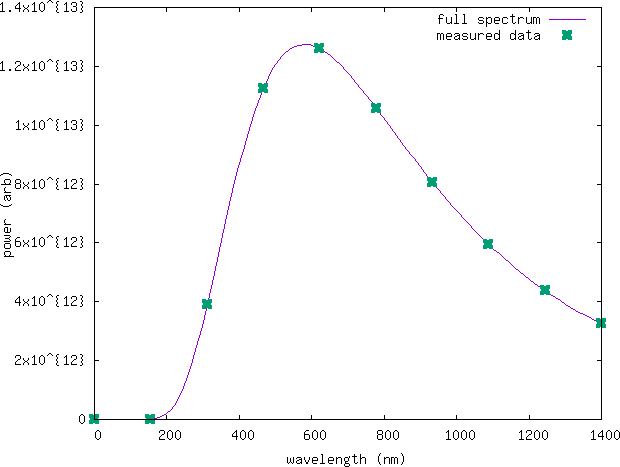
\includegraphics[width=4in]{spectrum-example.png}
  \caption{\label{fig:spectrum}An example of a measured power spectrum with the underlying full spectrum that is being measured}
\end{figure}
It is important to understand this in order to correctly determine the total power in the source. For a set of measurements, the total power
in the source will not just be the sum of the measured powers, but is instead the integral of the power spectrum that underlies the data. The total
power can be estimated from the measured data, but this must be done with numerical integration.

Assume that we have a set of $M$ measured powers, $P_j^\prime$ at discrete
wavelengths $\lambda_j$ which are uniformly separated, $\lambda_{j+1} -
\lambda_j = \Delta \lambda$. We want to model this source with as a collection
of single wavelength lasers, and we want to just use one laser for each
measured data point $M=N$ (rather than using the data to approximate $p(\lambda)$ via interpolation or curve fitting).
What power should each laser in the collection have? The answer is that they should have the same total power as the true broadband
source.

Let's use a Riemann sum approximation for the total power based on the measured data,
\begin{equation}
  P = \int\limits_{0}^{\infty} p(\lambda) d\lambda \approx \sum_j P_j^\prime (\lambda_{j+1} - \lambda_j)
\end{equation}
Therefore, the power we use for each laser in our model should be the measured power times distance between wavelengths: $P_i = P_i^\prime \Delta \lambda$.



\end{document}

